\documentclass[10pt,a4paper]{article}

\usepackage[utf8]{inputenc}
\usepackage[margin=1.8cm,top=2.0cm,bottom=2.0cm]{geometry}
\usepackage{helvet}
\usepackage{mathptmx}
\usepackage{microtype}
\usepackage{graphicx}
\usepackage{amsmath,amssymb}
\usepackage{booktabs}
\usepackage{xcolor}
\usepackage{fancyhdr}
\usepackage{titlesec}
\usepackage{caption}
\usepackage{tcolorbox}
\usepackage{hyperref}

\renewcommand{\familydefault}{\sfdefault}

% Nature Partner Journals colors
\definecolor{npjblue}{RGB}{20, 60, 120}
\definecolor{npjgray}{RGB}{90, 100, 110}
\definecolor{npjlgt}{RGB}{245, 248, 252}

\hypersetup{
    colorlinks=true,
    linkcolor=npjblue,
    citecolor=npjblue,
    urlcolor=npjblue
}

\pagestyle{fancy}
\fancyhf{}
\fancyhead[L]{\fontsize{8bp}{10bp}\selectfont\textbf{npj $\mid$ microgravity} \hspace{0.5em}\textcolor{npjgray}{$\mid$ Supplementary Information}}
\fancyhead[R]{\fontsize{8bp}{10bp}\selectfont\textcolor{npjgray}{Barker \& Porterfield (2026)}}
\fancyfoot[C]{\fontsize{8bp}{10bp}\selectfont\thepage}
\renewcommand{\headrulewidth}{0.4pt}
\renewcommand{\footrulewidth}{0.0pt}

\captionsetup{
    font={small,sf},
    labelfont={bf,sf},
    labelsep=period,
    justification=justified,
    singlelinecheck=false
}

\titleformat{\section}{\fontsize{12bp}{14bp}\bfseries\sffamily\color{npjblue}}{\thesection}{1em}{}
\titleformat{\subsection}{\fontsize{10bp}{12bp}\bfseries\sffamily}{\thesubsection}{1em}{}

\begin{document}

% -------------------------------------------------------------
% Title & Masthead
% -------------------------------------------------------------
\begin{tcolorbox}[colback=npjlgt,colframe=npjblue,arc=2mm,boxrule=1pt,left=5mm,right=5mm,top=4mm,bottom=4mm]
  \noindent{\fontsize{16bp}{18bp}\selectfont\textbf{\textsf{Supplementary Information}}}\\[4pt]
  {\fontsize{11bp}{14bp}\selectfont\textbf{Multiscale 3D cellular digital twin of a 164-seed plant community in the Artemis III LEAF growth chamber: microclimate CFD, foliar crowding, and substrate boundary layer dynamics}}\\[6pt]
  {\fontsize{9bp}{11bp}\selectfont Richard Barker\textsuperscript{1*} \& D. Marshall Porterfield\textsuperscript{1}}\\[2pt]
  {\fontsize{8bp}{10bp}\selectfont\textit{\textsuperscript{1}Department of Agricultural and Biological Engineering, Purdue University, West Lafayette, IN 47907, USA.}}\\[2pt]
  {\fontsize{8bp}{10bp}\selectfont\textit{*Corresponding author: barkerrj@purdue.edu}}
\end{tcolorbox}

\vspace{1em}

\noindent\textbf{Contents}:
\begin{itemize}
    \item \textbf{Supplementary Figure S1}: Gravitational Scaling \& Statolith-Mediated Root Phenotypes ($1.0g \to 0.38g \to 0.166g \to 0.0g$).
    \item \textbf{Supplementary Figure S2}: Hardware Ventilation Modes, CFD Streamlines, \& Ethylene Triple Response Phenotypes.
    \item \textbf{Supplementary Figure S3}: Substrate Hydraulic Potential \& Water Deficit Phenotypic Plasticity.
    \item \textbf{Supplementary Figure S4}: Sowing Density Sweeps \& Shade-Avoidance Phenotypic Plasticity ($0.25\times \to 2.0\times$).
    \item \textbf{Supplementary Figure S5}: Deep Space Ionizing Radiation \& Multi-Factor Stress Interaction Matrix.
    \item \textbf{Supplementary Note 1}: Mathematical Solvers \& Numerical Integration Parameters.
\end{itemize}

\clearpage

% -------------------------------------------------------------
% Supplementary Figure S1
% -------------------------------------------------------------
\begin{figure*}[p]
\centering
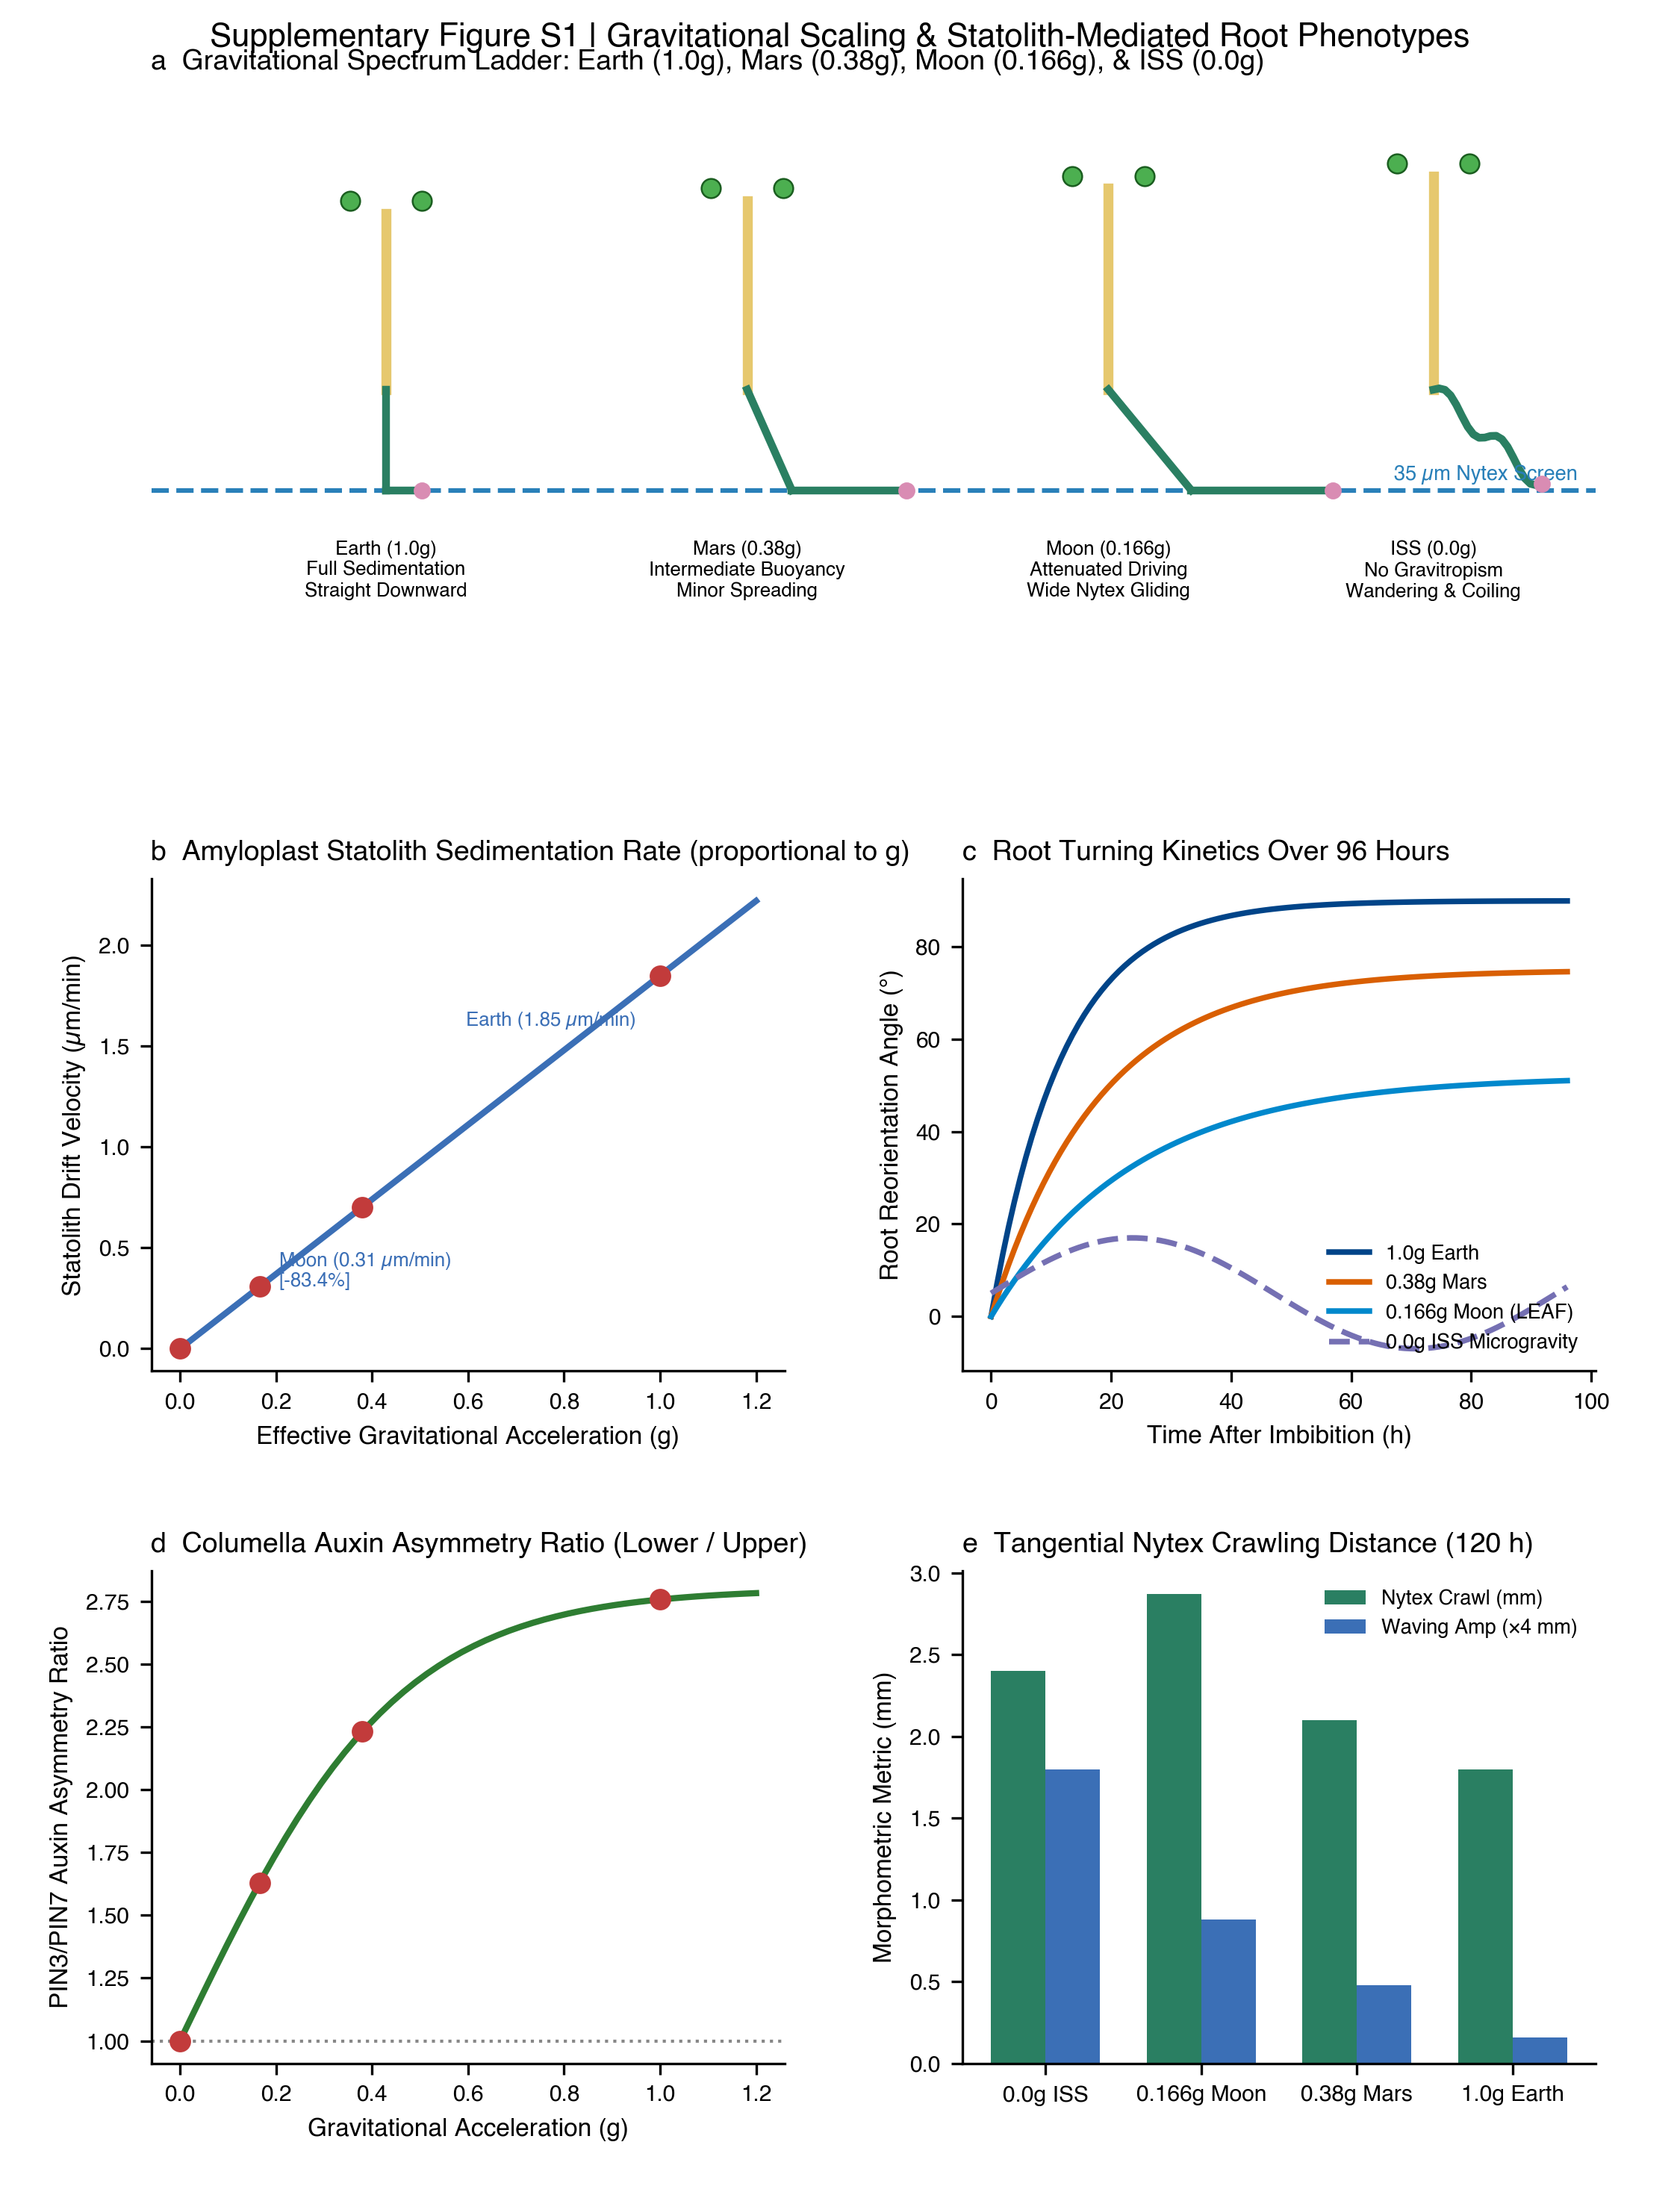
\includegraphics[width=\textwidth,height=0.72\textheight,keepaspectratio]{figS1_gravity_scaling_statolith_phenotypes.png}
\caption{\textbf{Gravitational scaling and statolith-mediated root phenotypic plasticity across Earth (1.0g), Mars (0.38g), Moon (0.166g), and ISS microgravity (0.0g).} 
\textbf{a}, Gravitational spectrum ladder displaying comparative seedling organ profiles. On Earth (1.0g), rapid amyloplast sedimentation establishes a strong downward gravitropic vector, leading to uniaxial downward penetration to the 35~$\mu$m Nytex screen. On Mars (0.38g) and the Moon (0.166g), sedimentation rate is attenuated by 62\% and 83.4\%, respectively, yielding delayed turning, wider radial dispersion ($35^\circ$), and extensive tangential gliding along the screen surface. In microgravity (0.0g), absence of statolith sedimentation produces stochastic root waving, autotropism, and contact-mediated thigmotropic coiling.
\textbf{b}, Linear scaling of amyloplast sedimentation velocity $v_{\mathrm{sed}}$ proportional to effective gravity $g$, dropping from $1.85\ \mu\mathrm{m\,min^{-1}}$ (Earth) to $0.31\ \mu\mathrm{m\,min^{-1}}$ (Moon).
\textbf{c}, Dynamic root tip turning kinetics $\theta_{\mathrm{root}}(t)$ over 96 hours post-imbibition.
\textbf{d}, Columella PIN3/PIN7 auxin asymmetry ratio (lower:upper statocyte membrane) saturating toward 2.8 at 1.0g and remaining unity (1.0) under microgravity.
\textbf{e}, Tangential Nytex crawl distance (reaching $2.87\ \mathrm{mm}$ on the Moon) and waving amplitude.}\label{fig:S1}
\end{figure*}

\clearpage

% -------------------------------------------------------------
% Supplementary Figure S2
% -------------------------------------------------------------
\begin{figure*}[p]
\centering
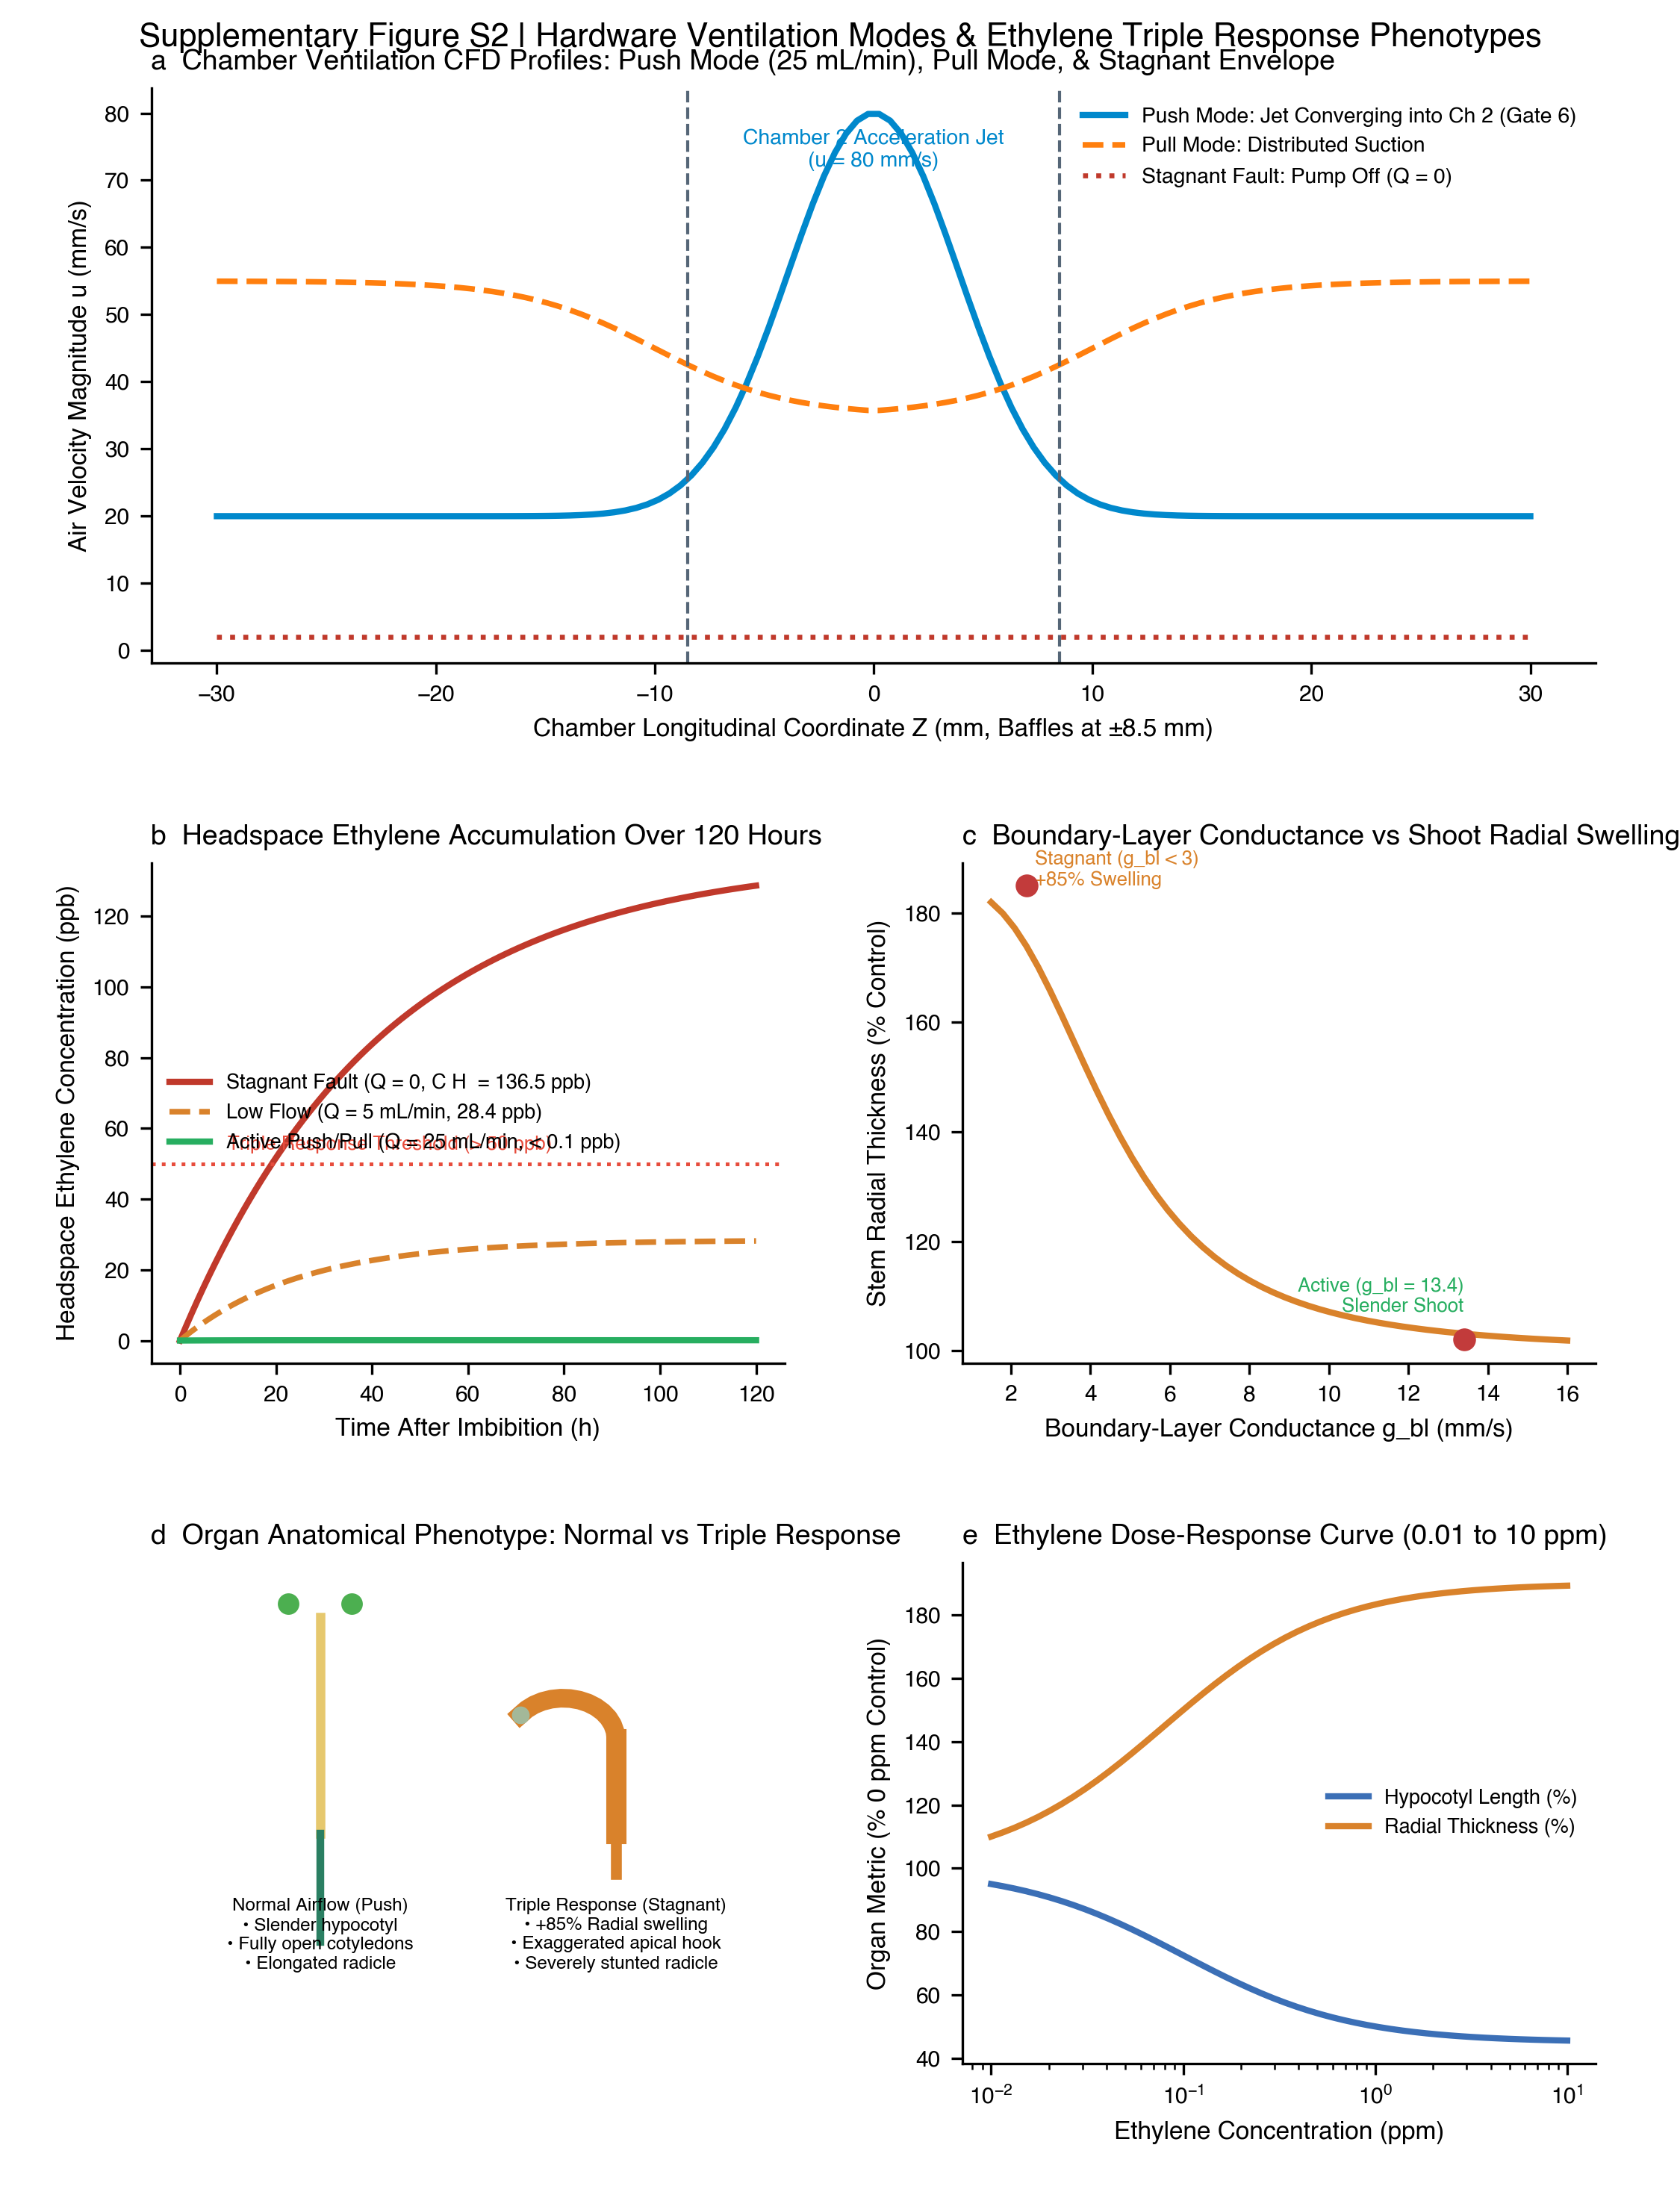
\includegraphics[width=\textwidth,height=0.72\textheight,keepaspectratio]{figS2_airflow_cfd_ethylene_triple_response.png}
\caption{\textbf{Hardware ventilation modes, chamber CFD airflow fields, and ethylene triple response phenotypes.}
\textbf{a}, 3D CFD air velocity magnitude profiles across the longitudinal coordinate $Z$ for Push mode ($Q = 25\ \mathrm{mL\,min^{-1}}$), Pull mode ($Q = 25\ \mathrm{mL\,min^{-1}}$), and Stagnant fault ($Q = 0$). Push mode creates a characteristic ``dip-and-converge'' jet through $Z = \pm 8.5\ \mathrm{mm}$ baffle windows, accelerating air velocity to $80\ \mathrm{mm\,s^{-1}}$ into Central Chamber 2.
\textbf{b}, Headspace ethylene accumulation dynamics over 120 hours. Active sweeping purges respiratory ethylene to $< 0.1\ \mathrm{ppb}$, whereas stagnant faults result in accumulation to $136.5\ \mathrm{ppb}$, far exceeding the $50\ \mathrm{ppb}$ triple response threshold.
\textbf{c}, Boundary-layer conductance $g_{\mathrm{bl}}$ plotted against hypocotyl radial swelling. In stagnant air ($g_{\mathrm{bl}} < 3\ \mathrm{mm\,s^{-1}}$), gas diffusion resistance traps ethylene in the boundary-layer envelope, triggering radial expansion.
\textbf{d}, Cellular organ anatomical phenotypes comparing slender, elongated seedlings in active airflow against the diagnostic triple response (swollen hypocotyl, exaggerated hook, stunted radicle) in stagnant air.
\textbf{e}, Dose-response curves of hypocotyl length and radial diameter across exogenous ethylene concentrations ($0.01$ to $10\ \mathrm{ppm}$).}\label{fig:S2}
\end{figure*}

\clearpage

% -------------------------------------------------------------
% Supplementary Figure S3
% -------------------------------------------------------------
\begin{figure*}[p]
\centering
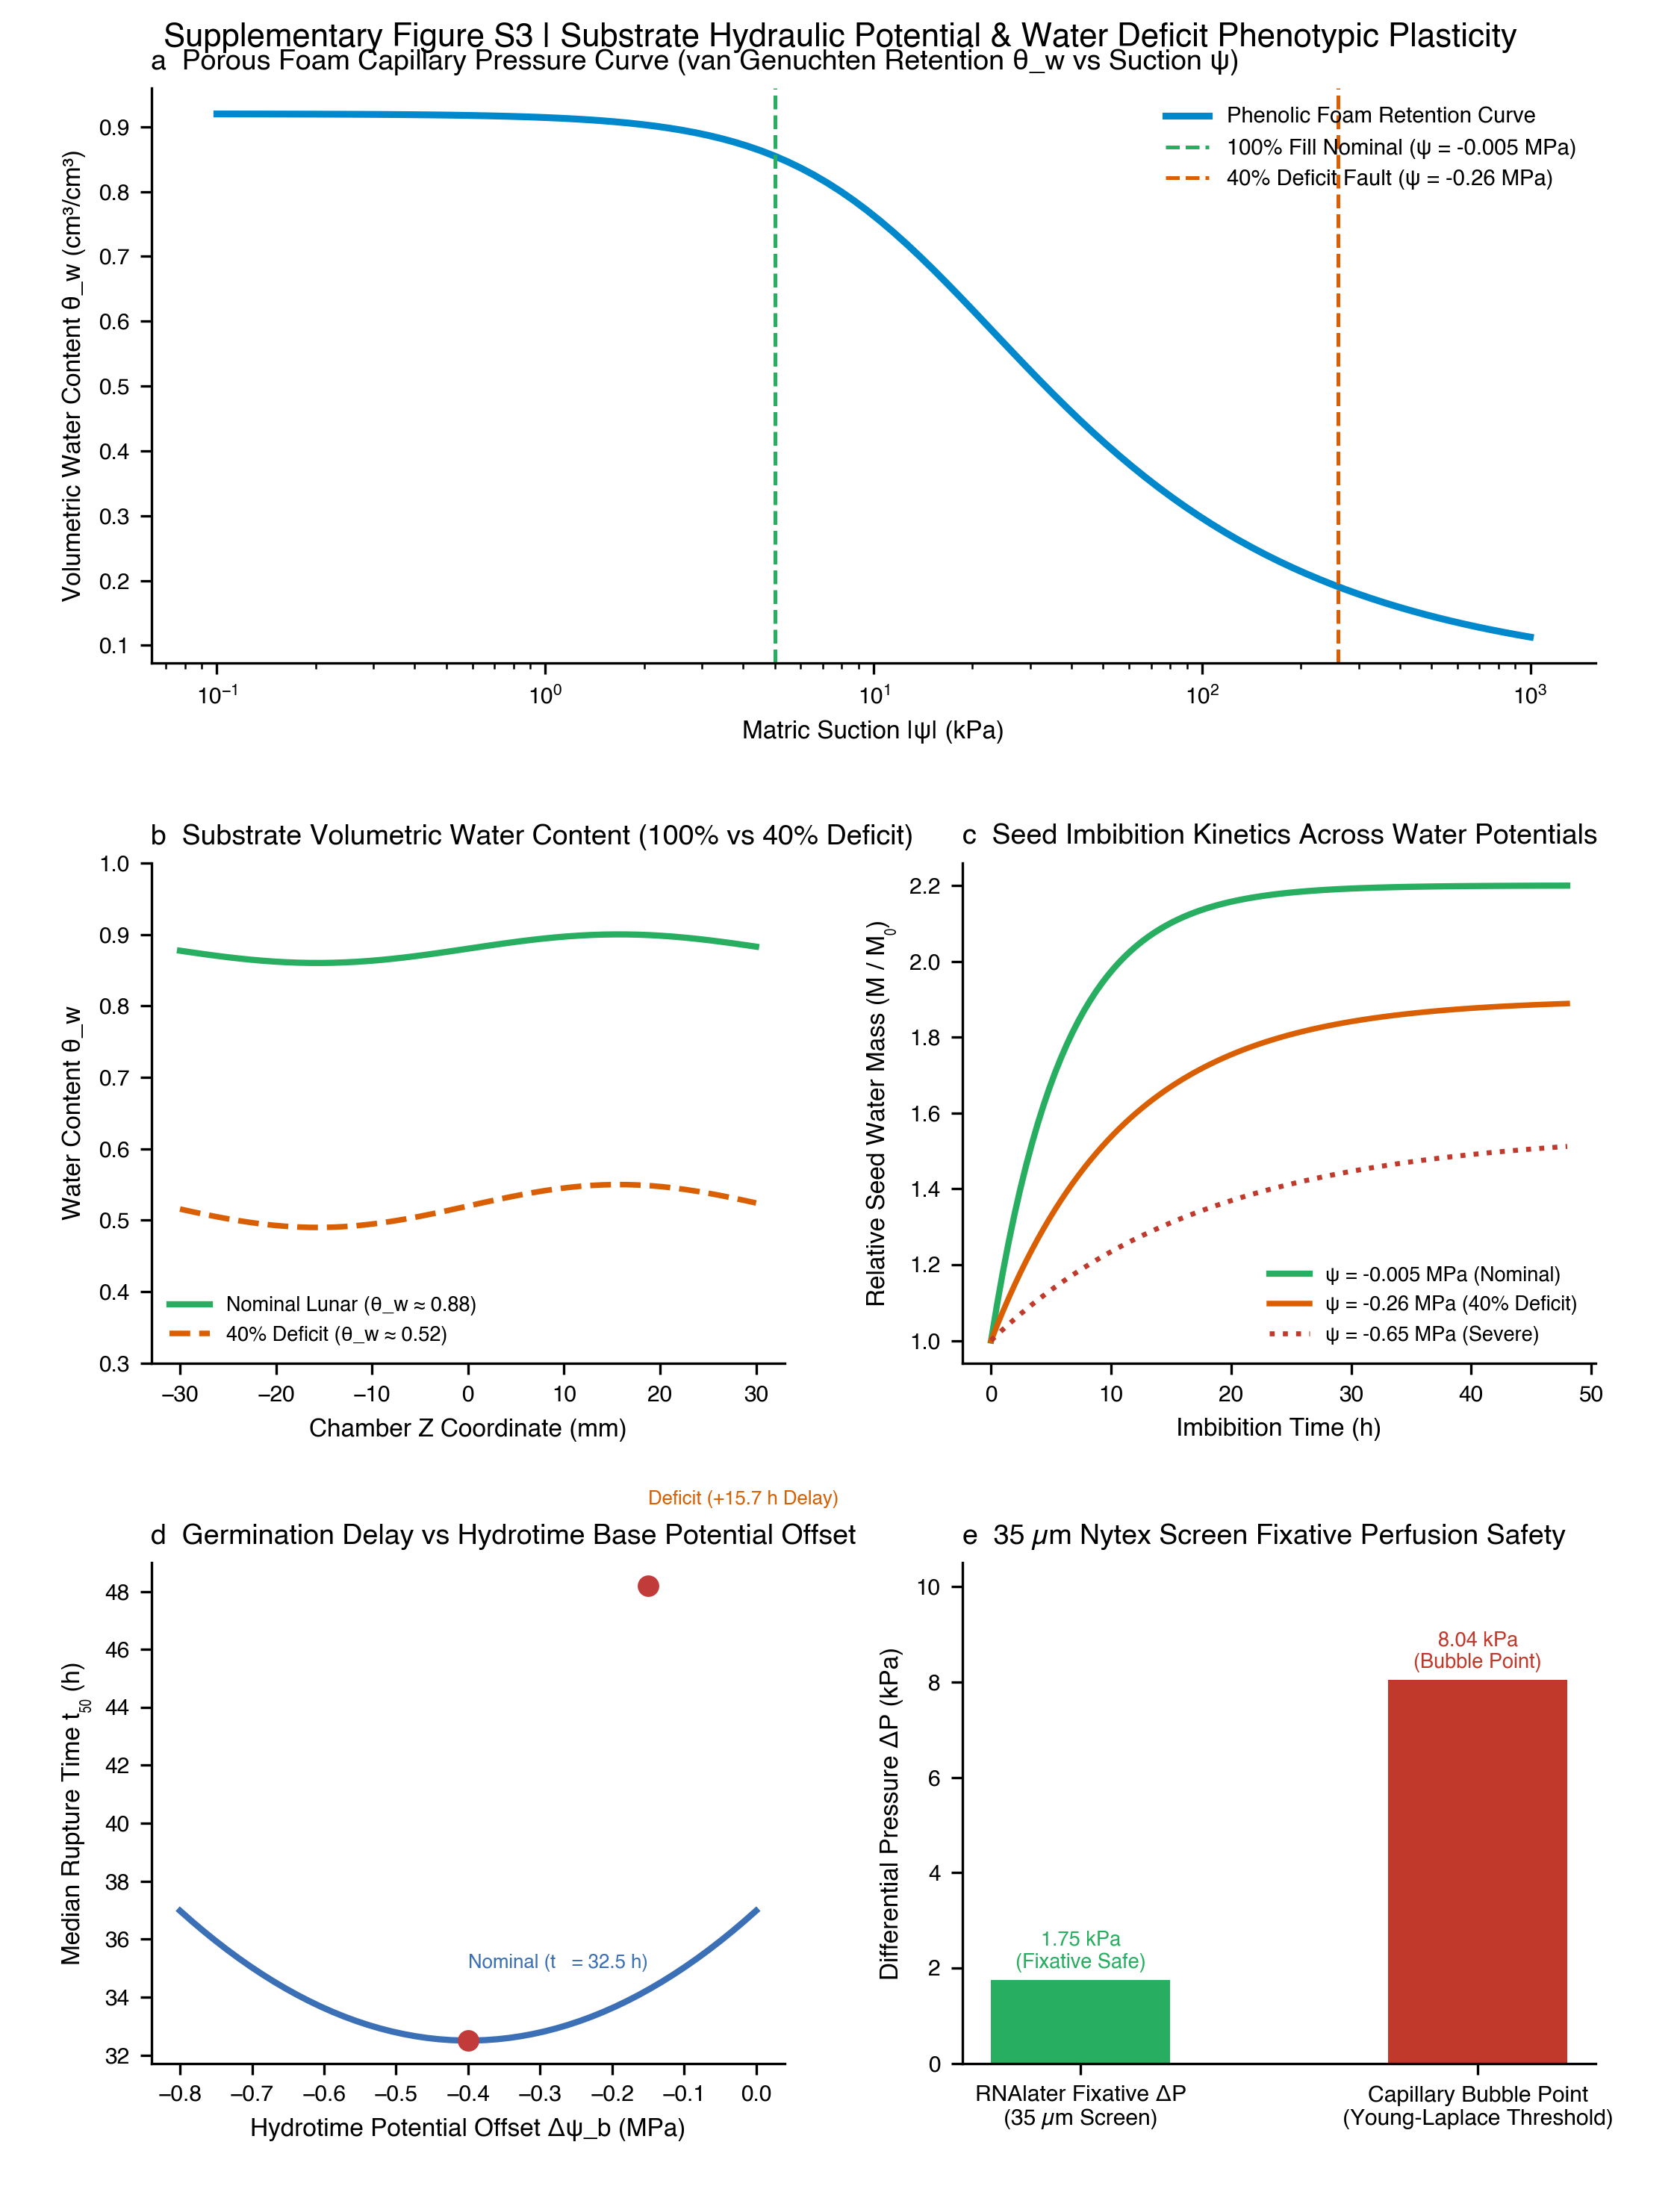
\includegraphics[width=\textwidth,height=0.72\textheight,keepaspectratio]{figS3_foam_capillary_hydration_deficit.png}
\caption{\textbf{Substrate hydraulic potential, van Genuchten retention, and water deficit phenotypic plasticity.}
\textbf{a}, Phenolic/polyurethane foam capillary retention curve modeled via the van Genuchten equation ($S_e = [1 + (\alpha |\psi|)^n]^{-m}$ with $\alpha = 0.08\ \mathrm{kPa^{-1}}$, $n = 1.6$). Nominal 100\% activation corresponds to $\psi = -0.005\ \mathrm{MPa}$, whereas a 40\% moisture deficit drops matric potential to $\psi = -0.26\ \mathrm{MPa}$.
\textbf{b}, Volumetric water content $\theta_w(z)$ along the foam slab under nominal ($\theta_w \approx 0.88$) versus deficit ($\theta_w \approx 0.52$) conditions.
\textbf{c}, Seed imbibition water mass uptake curves $M(t)/M_0$ across water potentials, showing delayed hydration plateaus under water stress.
\textbf{d}, Population germination delay as a function of the hydrotime base water-potential offset $\Delta \psi_b$, yielding a $+15.7\ \mathrm{h}$ median rupture delay under deficit.
\textbf{e}, 35~$\mu$m Nytex screen bubble-point capillary safety threshold: Young--Laplace capillary entry pressure ($\Delta P_{\mathrm{bubble}} = 8.04\ \mathrm{kPa}$) provides a four-fold safety margin over the end-of-mission RNAlater perfusion pressure drop ($\Delta P = 1.75\ \mathrm{kPa}$), ensuring zero foam intrusion.}\label{fig:S3}
\end{figure*}

\clearpage

% -------------------------------------------------------------
% Supplementary Figure S4
% -------------------------------------------------------------
\begin{figure*}[p]
\centering
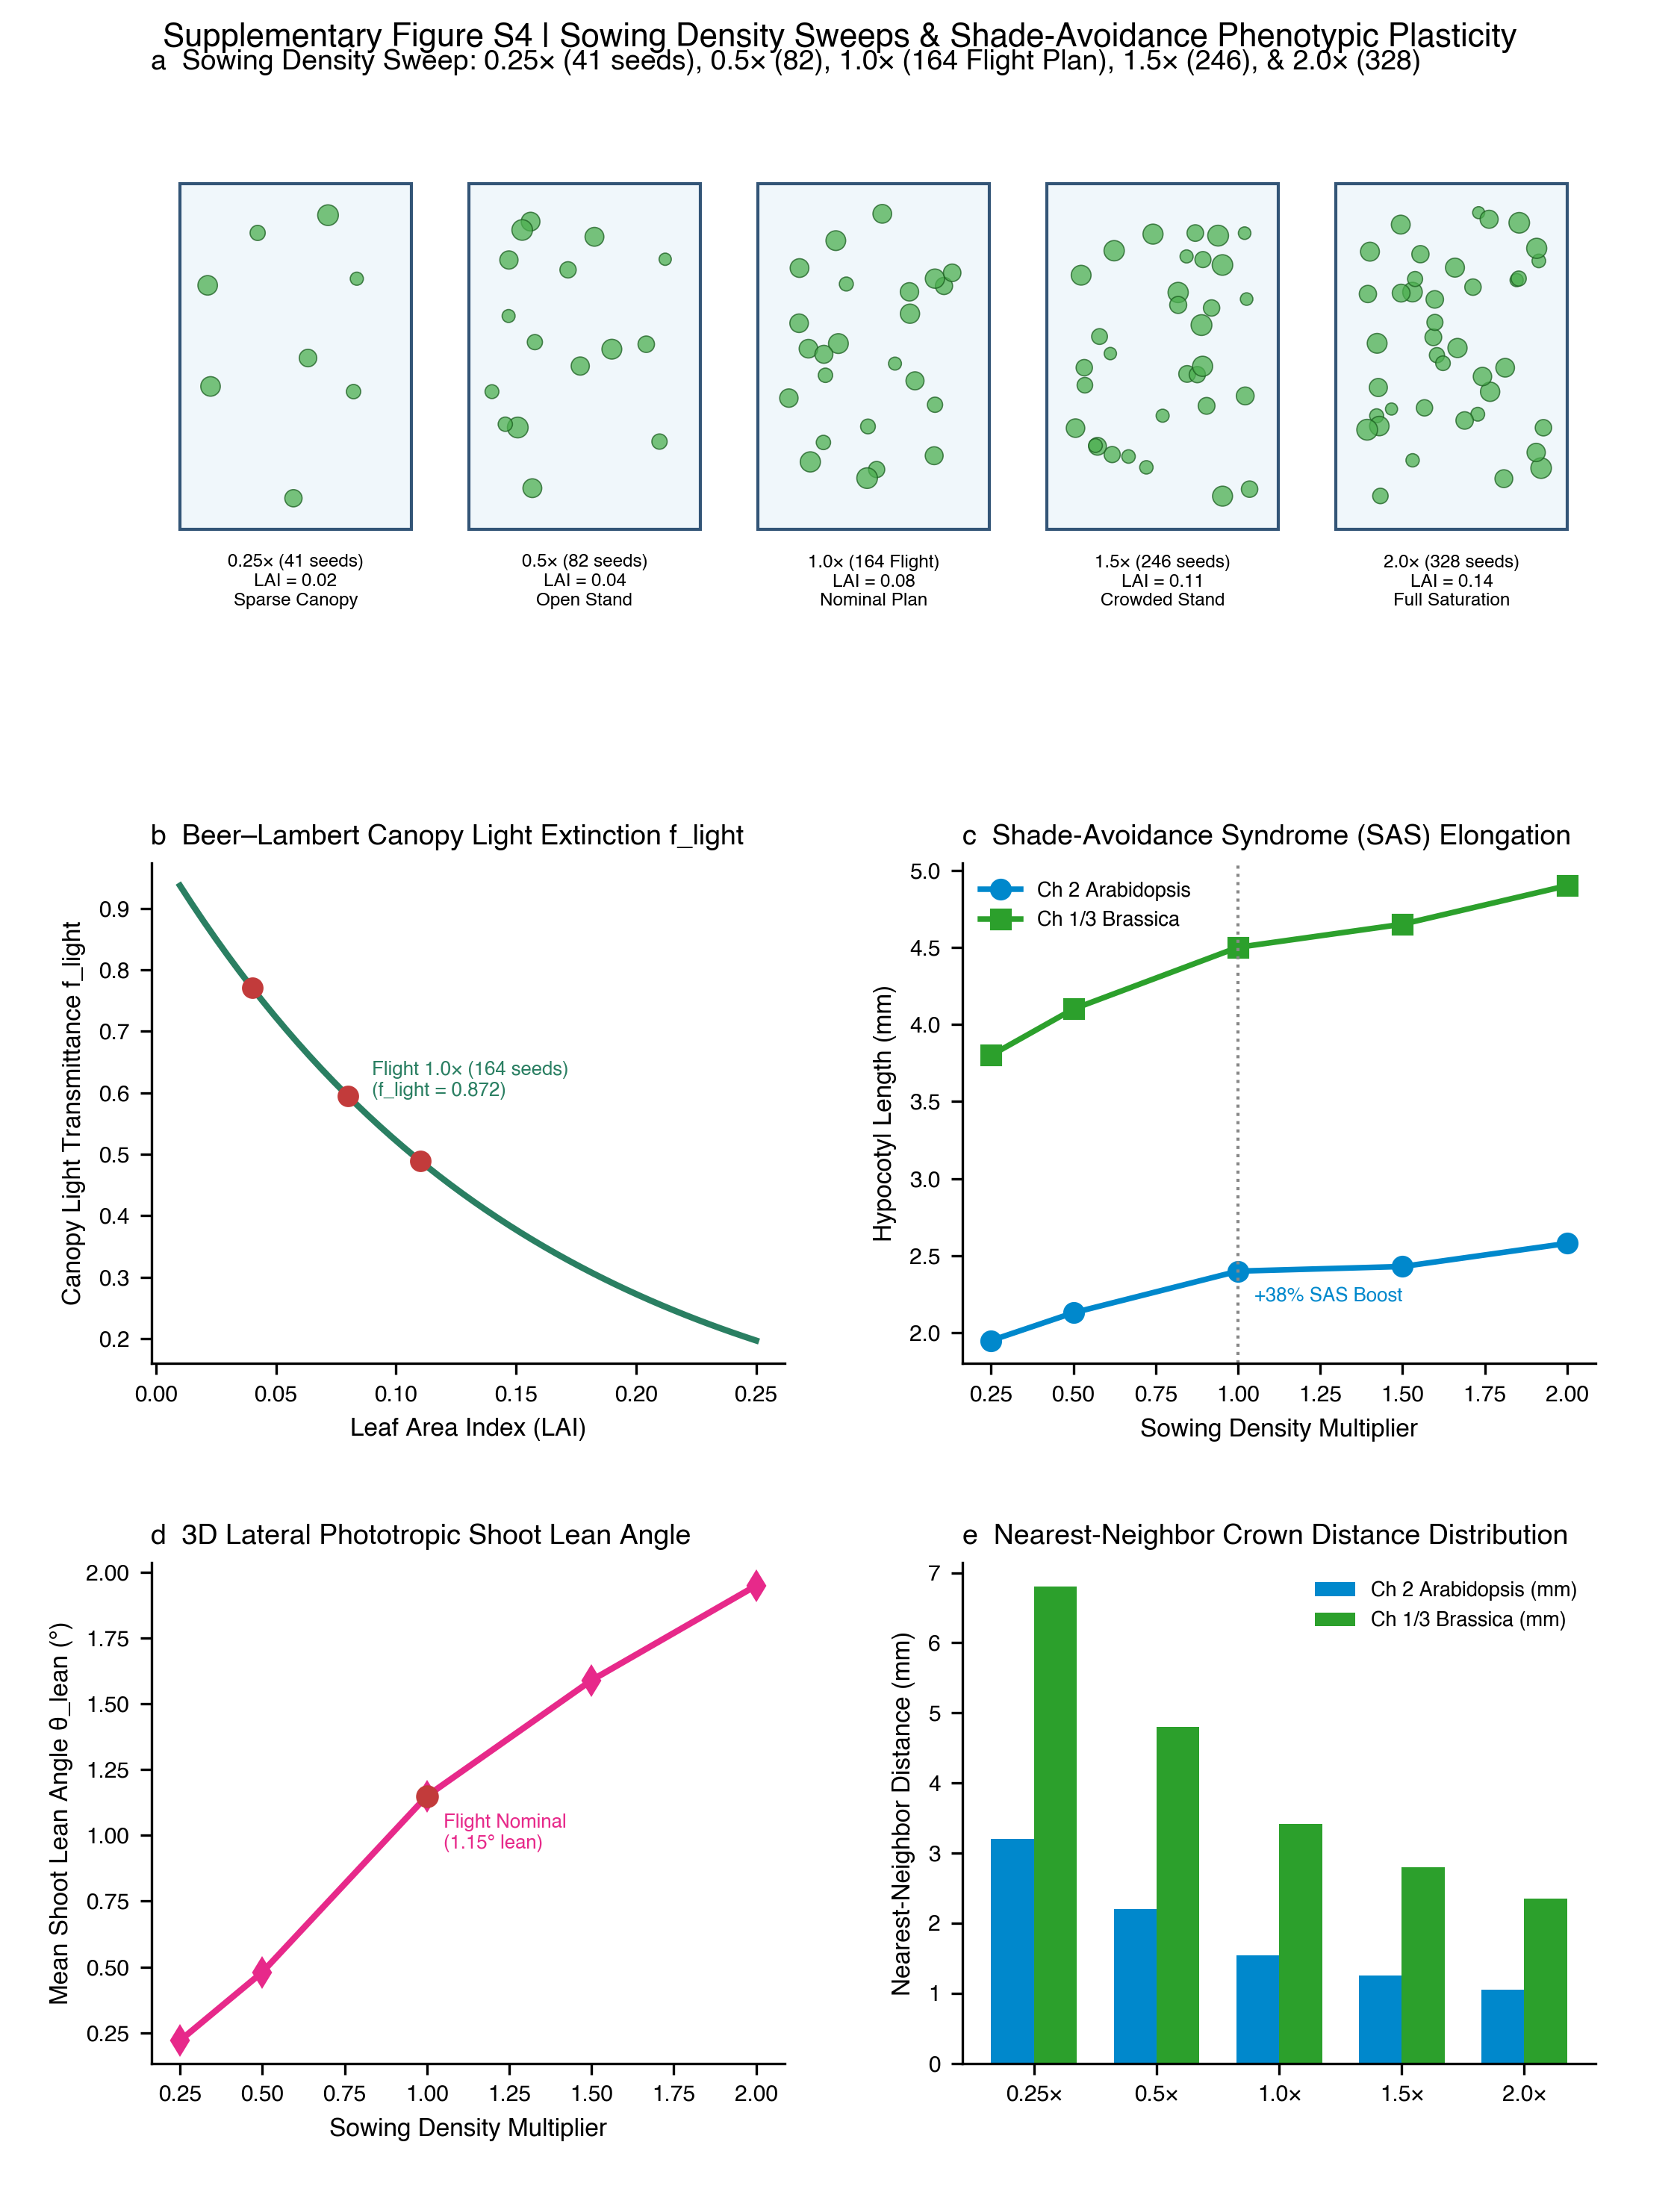
\includegraphics[width=\textwidth,height=0.72\textheight,keepaspectratio]{figS4_sowing_density_shade_avoidance_phototropism.png}
\caption{\textbf{Sowing density sweeps and shade-avoidance syndrome (SAS) phenotypic plasticity ($0.25\times$ to $2.0\times$ flight density).}
\textbf{a}, Top-down sowing architecture maps across 41 seeds ($0.25\times$), 82 seeds ($0.5\times$), 164 seeds ($1.0\times$ nominal flight plan), 246 seeds ($1.5\times$), and 328 seeds ($2.0\times$ saturation).
\textbf{b}, Beer--Lambert foliar canopy light extinction: canopy light transmittance $f_{\mathrm{light}} = \exp(-k \cdot LAI)$ decreasing from $0.943$ (sparse) to $0.815$ (crowded).
\textbf{c}, Shade-avoidance hypocotyl elongation response curve: low red:far-red ratio ($R:\mathrm{FR} < 0.35$) inactivates phytochrome B, stimulating auxin biosynthesis and driving a $+38\%$ hypocotyl elongation in Chamber 2 \textit{Arabidopsis}.
\textbf{d}, Lateral 3D phototropic shoot lean angle $\theta_{\mathrm{lean}}$ away from neighboring crowns, increasing monotonically from $0.22^\circ$ in sparse stands to $1.95^\circ$ at $2.0\times$ density.
\textbf{e}, Nearest-neighbor crown distance ($nnd$) distributions across species compartments.}\label{fig:S4}
\end{figure*}

\clearpage

% -------------------------------------------------------------
% Supplementary Figure S5
% -------------------------------------------------------------
\begin{figure*}[p]
\centering
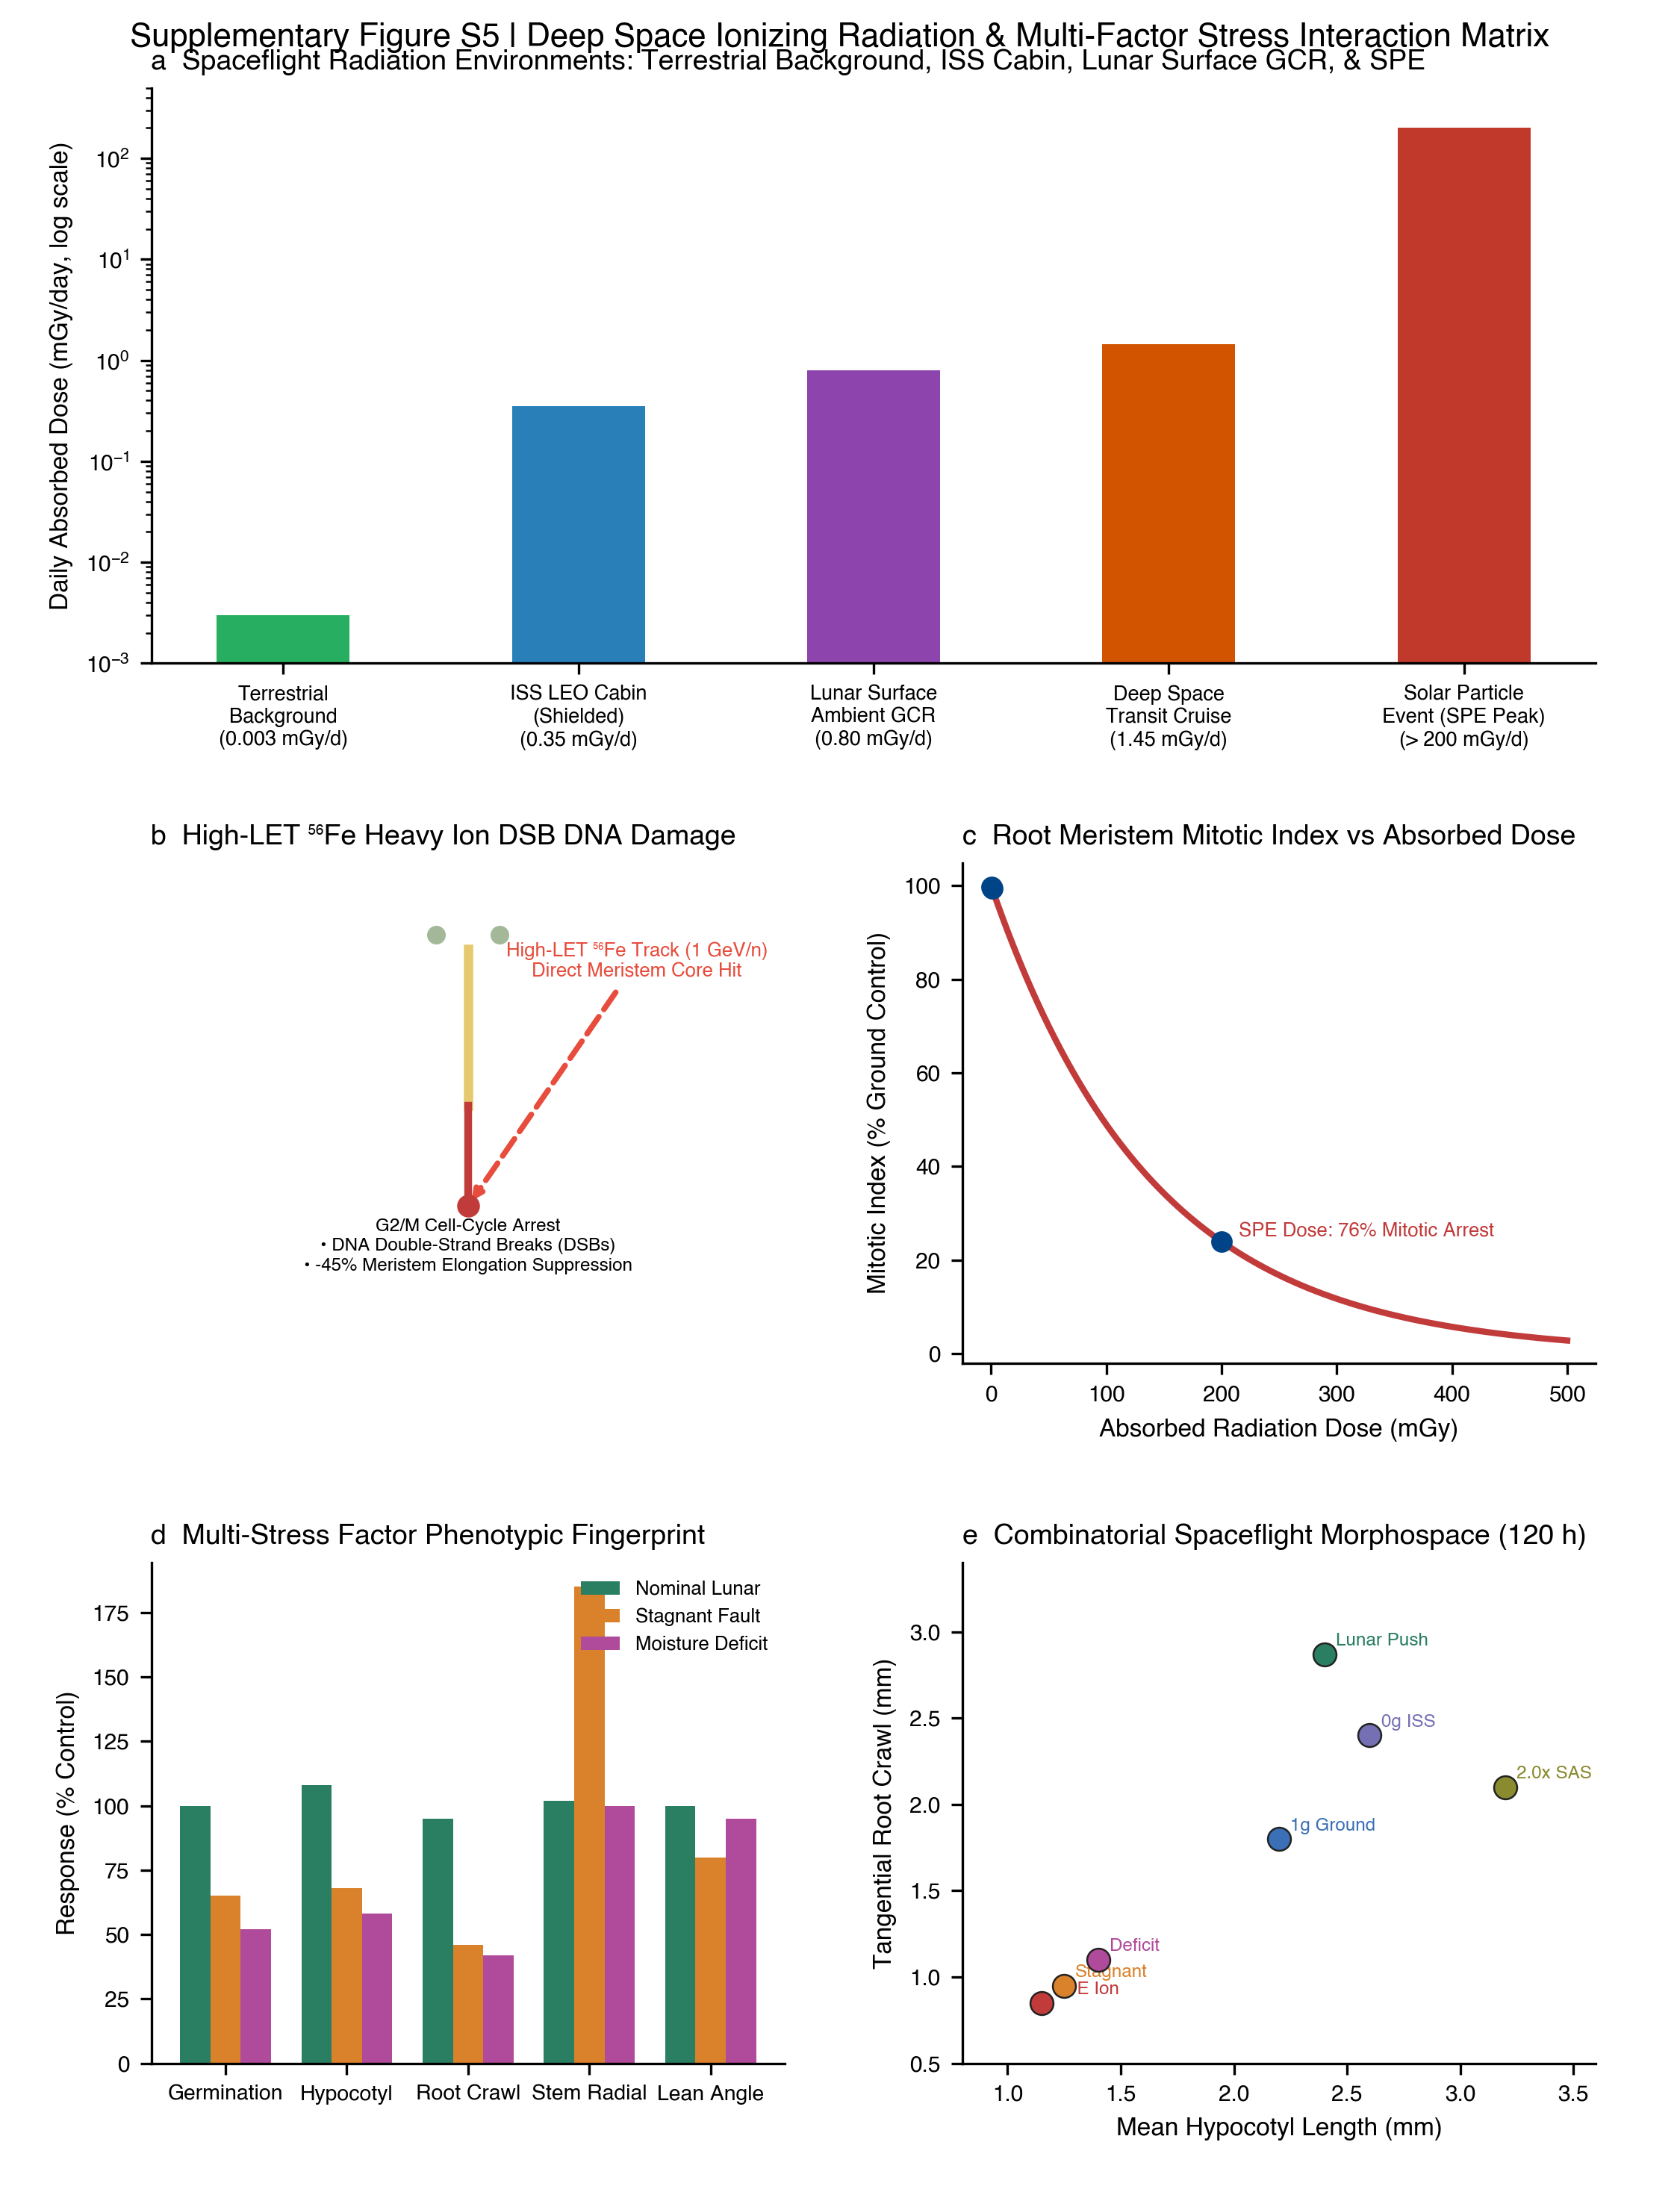
\includegraphics[width=\textwidth,height=0.72\textheight,keepaspectratio]{figS5_deepspace_radiation_stress_matrix.png}
\caption{\textbf{Deep space ionizing radiation and multi-factor spaceflight stress interaction matrix.}
\textbf{a}, Benchmark daily absorbed radiation doses across terrestrial background ($0.003\ \mathrm{mGy\,d^{-1}}$), ISS LEO cabin ($0.35\ \mathrm{mGy\,d^{-1}}$), lunar surface ambient GCR ($0.80\ \mathrm{mGy\,d^{-1}}$), deep space transit ($1.45\ \mathrm{mGy\,d^{-1}}$), and peak Solar Particle Events ($> 200\ \mathrm{mGy\,d^{-1}}$).
\textbf{b}, High-LET $^{56}\mathrm{Fe}$ heavy ion track structure (1~$\mathrm{GeV/n}$) passing through the seed meristem core, inducing localized clusters of DNA double-strand breaks (DSBs) and triggering the G2/M cell-cycle checkpoint.
\textbf{c}, Root apical meristem mitotic index suppression curve as a function of absorbed dose, showing 76\% mitotic arrest under SPE doses.
\textbf{d}, Multi-stress biometric radar comparing germination rate, hypocotyl length, root Nytex crawl, stem thickness, and lean angle across nominal lunar flight, stagnant pump-off faults, and moisture deficit.
\textbf{e}, Combinatorial spaceflight morphospace mapping 120-hour hypocotyl length against tangential root crawl across all mission vectors.}\label{fig:S5}
\end{figure*}

\clearpage

% -------------------------------------------------------------
% Supplementary Note 1
% -------------------------------------------------------------
\section*{Supplementary Note 1: Mathematical Solvers \& Physical Provenance}

The LEAF GBC1 digital twin couples continuous partial differential equations (PDEs), ordinary differential equations (ODEs), and discrete single-seed agent automata across all 164 individual seedlings.

\subsection*{1. Abley Bistable ABA--GA Integrator Hormone ODEs}
Each embryonic cell $i$ integrates intracellular abscisic acid ($A$), gibberellin ($G$), and DELLA ($D$) balances:
\begin{align}
\frac{dA_i}{dt} &= k_{A,\mathrm{syn}} \frac{1}{1 + (G_i / K_{GA})^n} - k_{A,\mathrm{deg}} A_i\\
\frac{dG_i}{dt} &= k_{G,\mathrm{syn}} \frac{1}{1 + (A_i / K_{ABA})^m} - k_{G,\mathrm{deg}} G_i \frac{D_i}{K_D + D_i}\\
\frac{dD_i}{dt} &= k_{D,\mathrm{syn}} - k_{D,\mathrm{deg}} G_i D_i
\end{align}
where endosperm rupture occurs when accumulated DELLA repressor activity in the radicle tip drops below the critical threshold $D_{\mathrm{crit}} = 0.35$.

\subsection*{2. Lockhart Wall Expansion with Cell Restraint}
Axial cell elongation rate $\dot{\epsilon}_i$ is governed by effective turgor pressure $P_i$ exceeding the wall yield stress $\sigma_y$:
\begin{equation}
\dot{\epsilon}_i = \Phi \max\left(0,\, P_i - \sigma_{\mathrm{restraint},i} - \sigma_y\right)
\end{equation}
where $\Phi$ is cell wall extensibility ($\mathrm{MPa^{-1}\,h^{-1}}$) and $\sigma_{\mathrm{restraint}}$ represents the mechanical containment exerted by the single-layer endosperm and outer testa coat prior to rupture.

\subsection*{3. Boundary-Layer Heat and Mass Transfer}
Convective boundary-layer conductance $g_{\mathrm{bl}}$ is resolved from the Nusselt/Sherwood correlations for laminar flow over a flat leaf of characteristic dimension $L$:
\begin{equation}
Sh = 2.0 + 0.6 \cdot Re_L^{1/2} Sc^{1/3},\quad g_{\mathrm{bl}} = \frac{D_v \cdot Sh}{L}
\end{equation}
where $D_v$ is binary gas diffusivity in air ($2.42 \times 10^{-5}\ \mathrm{m^2\,s^{-1}}$), $Re_L = u L / \nu$, and $Sc = \nu / D_v \approx 0.60$.

\subsection*{4. Young--Laplace Screen Bubble Point}
The critical capillary bubble-point entry pressure $\Delta P_{\mathrm{bubble}}$ for the 35~$\mu$m Nytex monofilament screen is:
\begin{equation}
\Delta P_{\mathrm{bubble}} = \frac{4 \gamma \cos \theta_c}{d_{\mathrm{pore}}}
\end{equation}
With surface tension $\gamma = 0.0728\ \mathrm{N\,m^{-1}}$, contact angle $\theta_c = 15^\circ$, and pore diameter $d_{\mathrm{pore}} = 35 \times 10^{-6}\ \mathrm{m}$, $\Delta P_{\mathrm{bubble}} = 8.04\ \mathrm{kPa}$. During terminal perfusion with RNAlater fixative ($\mu = 1.85\ \mathrm{mPa\,s}$), the Darcy flow pressure drop across the mesh is:
\begin{equation}
\Delta P = \frac{\mu Q_{\mathrm{perf}} \Delta y}{k_{\mathrm{mesh}} A_{\mathrm{screen}}} = 1.75\ \mathrm{kPa}
\end{equation}
providing a safety factor of $S = 8.04 / 1.75 = 4.59$, guaranteeing that the screen does not de-saturate and radicles do not intrude into the foam.

\end{document}
